% ++++++++++++ Controller PSoC Master klassen ++++++++++++++
\subsubsection{Domain-klasse: Data}

\begin{figure}[h]
\centering
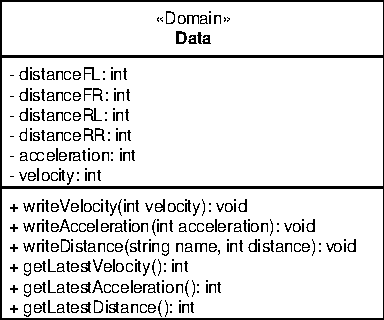
\includegraphics[]{../fig/diagrammer/bil/cd_data.pdf}
\caption{Klassebeskrivelse for domain-klassen Data}
\label{fig:cd_data}
\end{figure}

\textbf{Attributter}

\begin{table}[h]
\begin{tabularx}{\textwidth}{| Z | Z | L{10cm} |} \hline
Navn & Type & Beskrivelse \\\hline
\texttt{distanceFL} & \texttt{int} &Variabel der indeholder afstanden til en evt. forhindring ved forreste venstre hjørne af bilen i cm.\\\hline
\texttt{distanceFR} & \texttt{int} &Variabel der indeholder afstanden til en evt. forhindring ved forreste højre hjørne af bilen i cm.\\\hline
\texttt{distanceRL} & \texttt{int} &Variabel der indeholder afstanden til en evt. forhindring ved bageste venstre hjørne af bilen i cm.\\\hline
\texttt{distanceRR} & \texttt{int} &Variabel der indeholder afstanden til en evt. forhindring ved bageste højre hjørne af bilen i cm.\\\hline
\texttt{acceleration} & \texttt{int} &Variabel der indeholder bilens aktuelle acceleration i G.\\\hline
\texttt{velocity} & \texttt{int} &Variabel der indeholder bilens aktuelle hastighed i km/t.\\\hline
\end{tabularx}
\caption{Attributter for klassen Data}
\label{table:attr_data}
\end{table}
%TODO ret enheder

\textbf{Metoder}

\begin{table}[h]
\begin{tabularx}{\textwidth}{| L{2.5 cm} | Z |} \hline
Prototype & \texttt{void writeVelocity(int velocity)} \\\hline
Parametre & \texttt{velocity} \newline Den hastighed der skal indlæses. \\\hline
Returværdi &  \texttt{void} \newline \\\hline
Beskrivelse & Metoden indlæser den nyeste værdi af hastigheden i datastrukturen. \\\hline
\end{tabularx}
\caption{Metodebeskrivelse for \texttt{writeVelocity}}
\label{table:met_writeVelocity}
\end{table}

\begin{table}[h]
\begin{tabularx}{\textwidth}{| L{2.5 cm} | Z |} \hline
Prototype & \texttt{void writeAcceleration(int acceleration)} \\\hline
Parametre & \texttt{acceleration} \newline Den acceleration der skal indlæses. \\\hline
Returværdi &  \texttt{void} \newline \\\hline
Beskrivelse & Metoden indlæser den nyeste værdi af accelerationen i datastrukturen. \\\hline
\end{tabularx}
\caption{Metodebeskrivelse for \texttt{writeAcceleration}}
\label{table:met_writeAcceleration}
\end{table}

\begin{table}[h]
\begin{tabularx}{\textwidth}{| L{2.5 cm} | Z |} \hline
Prototype & \texttt{void  writeDistance(string name, int distance)} \\\hline
Parametre & \texttt{name} \newline Navnet på den sensor som der skal indlæses data fra. Kan være FL, FR, RL eller RR. \newline \newline
			\texttt{distance} \newline
			Afstanden der fra den pågældende sensor der skal indlæses i datastrukturen.\\\hline
Returværdi &  \texttt{void} \newline \\\hline
Beskrivelse & Metoden indlæser den nyeste værdi af fra en vilkårlig afstandssensor i datastrukturen. \\\hline
\end{tabularx}
\caption{Metodebeskrivelse for \texttt{writeDistance}}
\label{table:met_writeDistance}
\end{table}

\begin{table}[h]
\begin{tabularx}{\textwidth}{| L{2.5 cm} | Z |} \hline
Prototype & \texttt{int getLatestVelocity()} \\\hline
Parametre &  ~\newline \\\hline
Returværdi &  \texttt{int} \newline Den nyeste hastighedsmåling. \\\hline
Beskrivelse & Metoden returnerer den nyeste hastighedsmåling der er indlæst i datastrukturen. \\\hline
\end{tabularx}
\caption{Metodebeskrivelse for \texttt{getLatestVelocity}}
\label{table:met_getLatestVelocity}
\end{table}

\begin{table}[h]
\begin{tabularx}{\textwidth}{| L{2.5 cm} | Z |} \hline
Prototype & \texttt{int getLatestAcceleration()} \\\hline
Parametre &  ~\newline \\\hline
Returværdi &  \texttt{int} \newline Den nyeste accelerationsmåling. \\\hline
Beskrivelse & Metoden returnerer den nyeste accelerationsmåling der er indlæst i datastrukturen. \\\hline
\end{tabularx}
\caption{Metodebeskrivelse for \texttt{getLatestAcceleration}}
\label{table:met_getLatestAcceleration}
\end{table}

\begin{table}[h]
\begin{tabularx}{\textwidth}{| L{2.5 cm} | Z |} \hline
Prototype & \texttt{int getLatestDistance(string name)} \\\hline
Parametre &  \texttt{name}\newline Navnet på den sensor som der ønskes data fra. Kan være FL, FR, RL eller RR.\\\hline
Returværdi &  \texttt{int} \newline Den nyeste afstandsmåling fra den angivne sensor. \\\hline
Beskrivelse & Metoden returnerer den nyeste afstandsmåling fra den angivne sensor. \\\hline
\end{tabularx}
\caption{Metodebeskrivelse for \texttt{getLatestDistance}}
\label{table:met_getLatestDistance}
\end{table}